\subsection{成果一：可运行的质量判别与边界输出}
\label{sec:gate-results}
\begin{table}[t]
\caption{质量判别器的构造留出诊断。20个新父配置共200例；故障140、无害40、范围未知20。}\label{tab:gate}
\centering\small
\begin{tabularx}{\columnwidth}{Xrrr}
\toprule
方法 & 检出/140 & 误报/40 & 弃权 \\
\midrule
文档均分阈值适配 & 0 & 0 & 0 \\
仅参数名 & 20 & 0 & 60 \\
标准库 argparse & 80 & 0 & 60 \\
去接口检查 & 60 & 0 & 140 \\
去完整性检查 & 100 & 0 & 100 \\
完整判别器 & 140 & 0 & 60 \\
\bottomrule
\end{tabularx}
\par\vspace{3pt}\raggedright\footnotesize 阈值为本研究适配，不是发表版SkillNet的复现。完整判别器的60次弃权含40个缺行为证据的无害例；静态一致不自动获得可用认证。
\end{table}

在按父配置留出的200个构造案例中，完整判别器检出140/140个已知机械故障，
40个无害对照无误报，60例保持弃权（表\ref{tab:gate}）。
标准库argparse检出80/140；增加的60例来自缺资源、版本变化和语法规则，
不能写成“接口解析优于标准库”。
去接口检查降至60/140、去完整性检查为100/140，分别说明模块的有限增量。
文档阈值适配未检出这些干预，不能据此断言所有模型评分无效。

在288次自建程序行为试验中，完整判别器保留三种满足登记套件的实现，并为九种缺陷实现给出失败见证。
仅接口与文档路线仍会放行九种错误实现；只做静态门禁则12种都缺少可用性证据。
因此实际成果是能输出“修复、被测范围通过、证据不足、超出已测范围”的程序，
以及反证和输入边界，而不是一个没有依据的好坏平均分。
288次输出来自12个实现、每个24输入；不是288个自然技能。

前一阶段同一判别器静态复核200个自然包，只对一个包给出三条已知参数冲突，其余199包仍为证据不足。
470条命令仍为134条静态一致、3条冲突、333条未知，包含79个无法解析入口的观察，未将其删除。
这是当时静态结果；本轮三个包的行为证据另列，未改写该冻结分母。自然包总体覆盖仍有限。
构造留出全检出与自然包低覆盖应同时呈现，不能只挑前者报告100\%准确。

\subsection{成果二：完整产物收益与强对照}
\label{sec:network-results}
\begin{table*}[t]
\caption{18节点可执行网络的全部主留出结果。每档均为128个输入，弃权按未完成计；三档均值以同一128任务为单位。}\label{tab:network-main}
\centering\small
\begin{tabularx}{\textwidth}{Xrrrr}
\toprule
策略 & 1.0倍 & 1.5倍 & 2.0倍 & 三档均值(\%) \\
\midrule
词法前五＋路径 & 8 & 8 & 8 & 6.25 \\
MMR 前五＋路径 & 8 & 56 & 56 & 31.25 \\
DPP 前五＋路径 & 8 & 56 & 56 & 31.25 \\
原生元数据最短路径 & 16 & 16 & 16 & 12.50 \\
人工固定流程 & 0 & 128 & 128 & 66.67 \\
全局证据过滤＋最短路径 & 0 & 64 & 64 & 33.33 \\
全局证据风险路径 & 0 & 128 & 128 & 66.67 \\
ECP 完整方法 & 16 & 128 & 128 & 70.83 \\
条件证据前五＋路径 & 4 & 88 & 88 & 46.88 \\
ECP 去版本绑定 & 16 & 128 & 128 & 70.83 \\
\bottomrule
\end{tabularx}
\par\vspace{3pt}\raggedright\footnotesize 预算锚为只用元数据求得的最低可行路径字节数，非根据测试成功选取。上下文字节不是LLM token或费用。人工流程与全局风险路径在两档宽预算上均与完整方法持平。
\end{table*}

表\ref{tab:network-main}给出全部策略和三档预算。
ECP完整方法的主估计为70.83\%，原生元数据最短路径12.50\%，配对差58.33个百分点；
人工固定与全局证据风险路径均为66.67\%，差值仅4.17个百分点。
相对元数据基线有224个预算案例改善、0个恶化、160个持平；
相对人工/全局风险均为16个改善、0个恶化、368个持平。
这些都是128任务在三档预算上的重复比较，不能按384个独立输入解释。

中预算下ECP、人工固定与全局风险均完成128/128。
ECP相对这两个强对照的主终点增量全部来自最紧预算：16/128对0/128。
所以不能写成宽预算下求解能力超过已知正确流程。
全局过滤后最短路径在中预算仅64/128；这表明只过滤已知坏节点仍可能把未探测变体选成便宜路径。
条件证据前五仅88/128，完整路径为128/128，说明在本网络中先保留互补能力再求路径比逐节点截断有效。
词法、MMR和DPP的较低数值只适用于当前表示与小网络，不能作为对训练路由器的优越性证明。

\begin{table}[t]
\caption{ECP相对各对照的三档平均成功差（百分点）。32个构造条件块的10,000次条件重采样；不作总体或多重检验显著性主张。}\label{tab:network-effects}
\centering\small
\begin{tabularx}{\columnwidth}{Xrr}
\toprule
对照 & 平均差 & 95\%条件区间 \\
\midrule
词法前五＋路径 & 64.58 & [58.31, 70.83] \\
MMR 前五＋路径 & 39.58 & [28.12, 50.00] \\
DPP 前五＋路径 & 39.58 & [29.17, 50.00] \\
原生元数据最短路径 & 58.33 & [50.00, 64.58] \\
人工固定流程 & 4.17 & [1.04, 8.33] \\
全局证据过滤＋最短路径 & 37.50 & [27.08, 47.92] \\
全局证据风险路径 & 4.17 & [1.04, 8.33] \\
条件证据前五＋路径 & 23.96 & [13.54, 34.38] \\
ECP 去版本绑定 & 0.00 & [0.00, 0.00] \\
\bottomrule
\end{tabularx}
\end{table}

\begin{figure*}[t]
\centering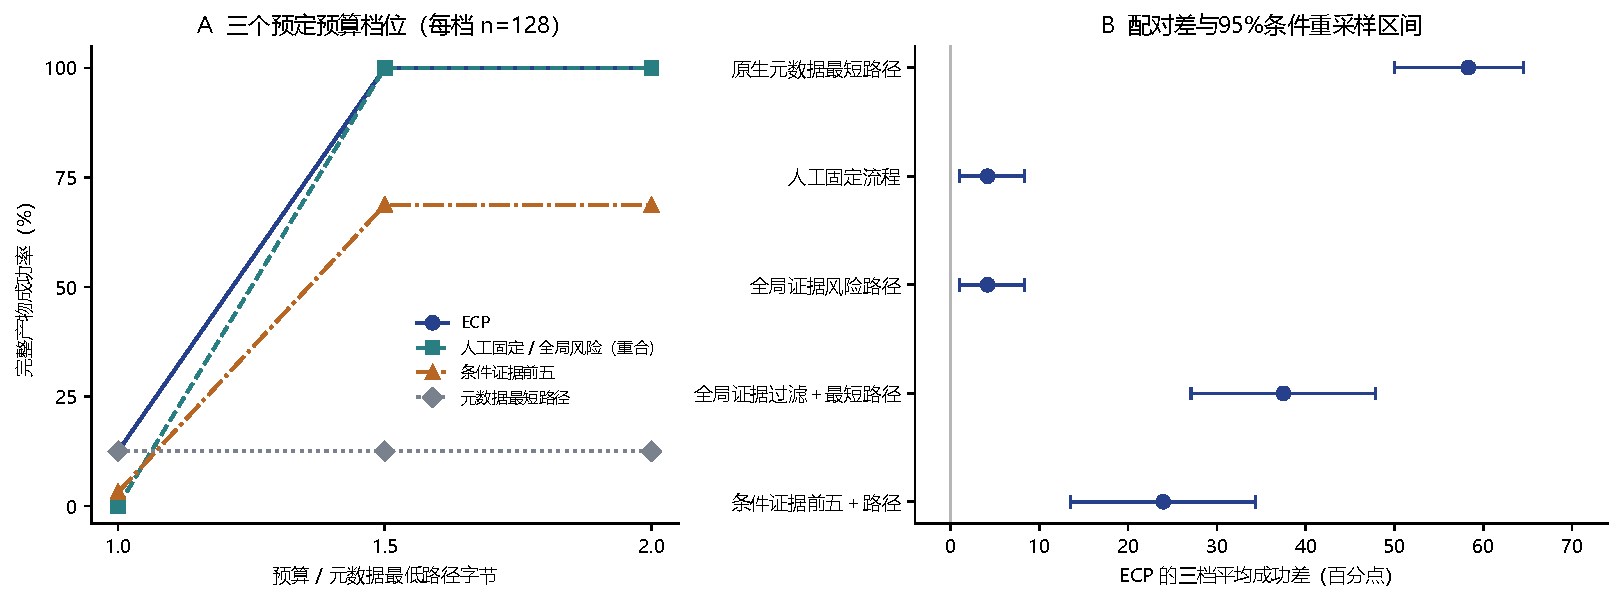
\includegraphics[width=.99\textwidth]{figures/network_budget_effects.pdf}
\caption{公开数据派生构造任务上的实际执行结果。左：预算不根据输出选取，点间连线仅辅助读图；人工固定与全局风险在三个主预算档重合。右：配对差的条件重采样区间，非标准误、非自然任务总体保证；颜色不编码显著性。}
\label{fig:network-budget}
\end{figure*}
表\ref{tab:network-effects}保留全部配对区间。
ECP相对元数据的95\%条件区间为[50.00,64.58]个百分点；
相对人工及全局风险均为[1.04,8.33]。
这描述当前32个构造条件块，不是已证实总体领先的概率。
两个留出数据集的每策略三档成功总数恰好相同（附表\ref{tab:network-datasets}），
说明受控语义和故障条件主导了差异，也限制了数据来源变化带来的外部效度。

\subsection{网络究竟改好了什么，成本是否值得}
\begin{table*}[t]
\caption{中预算资源与求解开销。包含失败尝试；前期取证为证据方法各自计入928次，非跨方法重复收费。}\label{tab:network-cost}
\centering\small
\begin{tabularx}{\textwidth}{Xrrrr}
\toprule
策略 & 成功/128 & 调用总数 & 上下文字节均值 & 含取证调用/成功 \\
\midrule
原生元数据最短路径 & 16 & 288 & 1801.5 & 18.00 \\
人工固定流程 & 128 & 448 & 2018.5 & 3.50 \\
全局证据过滤＋最短路径 & 64 & 448 & 1818.5 & 21.50 \\
全局证据风险路径 & 128 & 416 & 2023.5 & 10.50 \\
ECP 完整方法 & 128 & 416 & 1936.5 & 10.50 \\
\bottomrule
\end{tabularx}
\par\vspace{3pt}\raggedright\footnotesize 字节均值以启动路径为分母；本表五策略均启动128条。ECP含取证后为(416+928)/128=10.50，人工流程为448/128=3.50。调用不是货币成本。
\end{table*}

在同样完成128个中预算任务时，ECP用416次算子调用，人工流程448次，减少7.14\%；
平均上下文字节为1,936.5对2,018.5，减少4.06\%。
全局风险同为416次调用，但字节为2,023.5，ECP少4.30\%。
复合清洗与条件受限但适配的节点解释了这些变化；上下文字节仅是预先定义的资源代理，
复合节点按一次登记调用计，其内部三项操作未分别计价；
未实测CPU工作量、LLM token、端到端延迟或货币节省，不能替换成这些成本结论。

然而928次开发取证并非免费计算。
计入取证后，ECP本批为(416+928)/128=10.50次调用/正确产物，人工固定为3.50。
因此\emph{本批全成本不优于已知正确人工流程}。
若长期任务混合与版本稳定，按每任务节省0.25次调用粗略摊销，需约3,712个任务抵消探测调用；
这只是规划计算，未实测该规模，也没有计人工维护、探测异质成本和漂移后的重新取证。
方法是否值得采用，必须由新增覆盖、维护条件及完整成本决定。

\subsection{版本绑定的作用与不能组合的能力边界}
\begin{table*}[t]
\caption{固定压力实验及事后组合反例。各列均为中预算成功数。}\label{tab:network-stress}
\centering\small
\begin{tabularx}{\textwidth}{Xrrrr}
\toprule
策略 & 精度/24 & 换版本/128 & 缺能力/16 & 组合/24 \\
\midrule
词法前五＋路径 & 0 & 8 & 0 & 0 \\
MMR 前五＋路径 & 0 & 56 & 0 & 0 \\
DPP 前五＋路径 & 0 & 56 & 0 & 0 \\
原生元数据最短路径 & 0 & 16 & 0 & 0 \\
人工固定流程 & 24 & 64 & 0 & 12 \\
全局证据过滤＋最短路径 & 0 & 64 & 0 & 0 \\
全局证据风险路径 & 24 & 128 & 0 & 0 \\
ECP 完整方法 & 24 & 128 & 0 & 12 \\
条件证据前五＋路径 & 10 & 56 & 0 & 6 \\
ECP 去版本绑定 & 24 & 64 & 0 & 12 \\
\bottomrule
\end{tabularx}
\par\vspace{3pt}\raggedright\footnotesize 精度、换版本、缺能力在执行前固定；最右列为观察主结果后的证伪检查，复用同24个精度输入，不增加独立样本。组合条件中ECP只通过12/24，未据此调参。缺能力时全部方法弃权。
\end{table*}

替换已取证指标节点的代码但保留ID后，ECP与全局风险仍通过128/128，
仅按ID沿用旧证据的消融为64/128，人工固定也为64/128。
这支持资源版本匹配的必要性；因为全局风险同样成功，该收益不能全部归因于条件化。
去版本消融在无版本变化的主任务上与ECP完全一致，符合机制预期。

单独精度压力在中预算下，ECP、人工与全局风险均为24/24；最紧预算下ECP四次启动均失败。
进一步在观察主结果后合并精度与换版本，ECP只通过12/24，人工与去版本策略也为12/24，
全局风险为0/24（图\ref{fig:network-stress}）。
开发条件只区分是否存在0.5边界，没有编码任意小数精度；
无已知失败的候选也可能因浮点舍入失败。
这个反例说明单项压力通过不推出组合条件通过，平均组证据更不能变成整个输入族认证。
它作为事后证伪单列，未据此回调参数后冒充留出改进。

\begin{figure*}[t]
\centering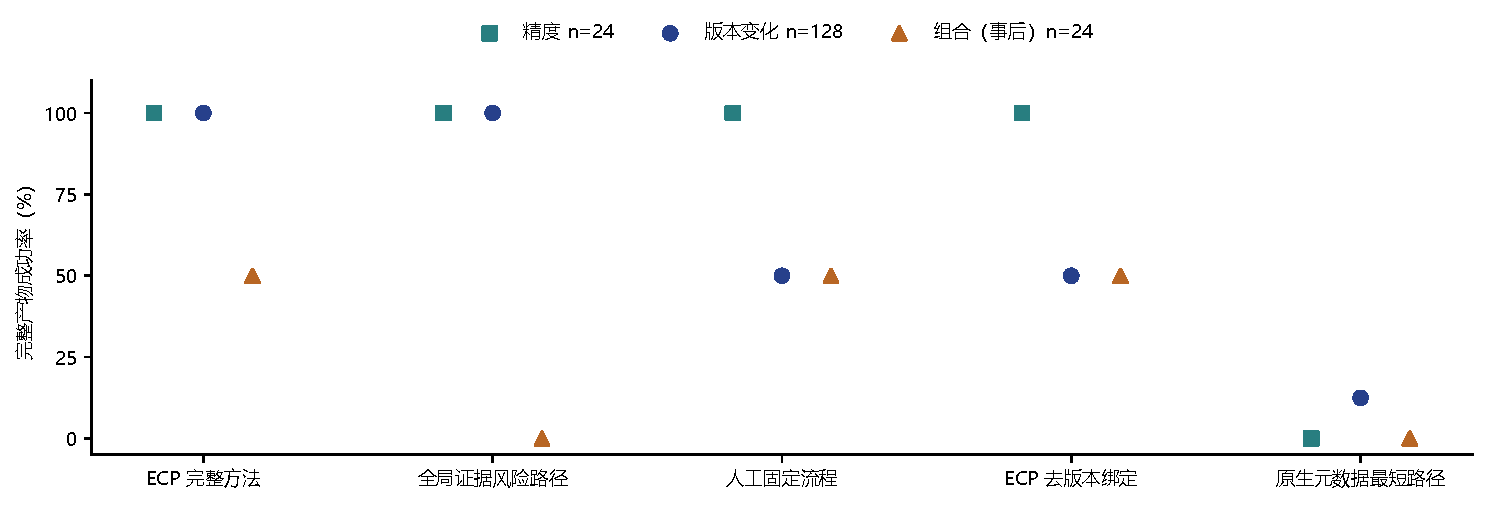
\includegraphics[width=.94\textwidth]{figures/network_stress.pdf}
\caption{中预算压力比较。不同列使用128或24个输入，各分母明确列出；组合压力为事后检查，复用24个精度输入。ECP单项均通过但组合只为50\%，是方法能力边界的实际反例。}
\label{fig:network-stress}
\end{figure*}
删除全部指标能力后，十种方法均弃权、成功均为零；这反映候选池上限，不是ECP特有优势。
三次ID置换后，ECP和全局风险均保持128/128、元数据16/128；MMR在40、16、24/128之间变化。
原始MMR为56/128，说明中性说明和并列顺序会影响词法截断。
置换仅为同输入敏感性检查，不能扩充主样本或证明任意命名下不变。
